\makeatletter
\makeatother\documentclass[10pt,english,oneside,twocolumn,a4paper]{article}% change 'a4paper' to 'letter' to use imperial paper format.
\usepackage{graphicx}
%% Font: Times
\usepackage[utf8]{inputenc}
\usepackage{mathptmx}
%\def\rmdefault{utm}
\usepackage{tabularx}
\usepackage{ragged2e}
\usepackage{todonotes}
\usepackage{flushend}
\usepackage[singlelinecheck=false]{caption}
\usepackage[T1]{fontenc}
\usepackage[numbers]{natbib}
\usepackage{amsmath}
\usepackage{babel}
\usetikzlibrary{calc,positioning}

\newcommand{\clash}{C$\lambda$aSH}

\pagestyle{empty}
\hoffset-1in
\voffset-1in
\oddsidemargin20truemm
\makeatletter
\let\ps@plain\ps@empty
\def\@xivpt{14pt}
\raggedbottom
\setcounter{secnumdepth}{4}
\columnsep5mm
\def\@sect#1#2#3#4#5#6[#7]#8{%
  \ifnum #2<2
    \null\par\vskip-15pt
  \fi
  \ifnum #2>\c@secnumdepth 
    \let\@svsec\@empty
  \else
    \refstepcounter{#1}%
    \protected@edef\@svsec{%
      \ifnum #2<4
        \hb@xt@10mm{\csname the#1\endcsname}\relax
      \else
        \hb@xt@12mm{\csname the#1\endcsname}\relax
      \fi}%
  \fi
  \@tempskipa #5\relax
  \ifdim \@tempskipa>\z@
    \begingroup
      #6{%
        \@hangfrom{\hskip #3\relax\@svsec}%
          \interlinepenalty \@M #8\@@par}%
    \endgroup
    \csname #1mark\endcsname{#7}%
    \addcontentsline{toc}{#1}{%
      \ifnum #2>\c@secnumdepth \else  
        \protect\numberline{\csname the#1\endcsname}%
      \fi 
      #7}%
  \else
    \def\@svsechd{%
      #6{\hskip #3\relax
      \@svsec #8}%
      \csname #1mark\endcsname{#7}%
      \addcontentsline{toc}{#1}{%
        \ifnum #2>\c@secnumdepth \else
          \protect\numberline{\csname the#1\endcsname}%
        \fi
        #7}}%
  \fi
  \@xsect{#5}}%
\renewcommand\LARGE{\@setfontsize\LARGE{16}{20}}
\renewcommand\abstract[2][Abstract]{\def\heading@abstract{#1}\def\@abstract{#2}}
\def\affil#1{\def\@affil{#1}}
%% Def. Titelei
\headheight0pt
\headsep0mm
\topskip10pt
\topmargin23mm
\textwidth170mm
\textheight58\baselineskip
\def\@maketitle{%
  \newpage
  \null
  \let \footnote \thanks
    {\addvspace{-5pt}\LARGE\bfseries\RaggedRight \@title \par}%
    \vskip 5.75mm%
    {\fontsize{12}{14}\selectfont
      % \lineskip 1ex%
      \@author,\space\@affil}%
    \vskip 15.75mm%
    {{\Large\bfseries\RaggedRight\heading@abstract}\par\vskip14pt
      \@abstract}%
  \par
  \vskip 4\baselineskip}

\renewcommand\section{\@startsection {section}{1}{\z@}%
                                   {-18pt}%
                                   {6pt}%
                                   {\Large\bfseries\RaggedRight}}
\renewcommand\subsection{\@startsection{subsection}{2}{\z@}%
                                     {10pt \@plus 1ex \@minus .2ex}%
                                     {2.5pt}%
                                     {\normalfont\large\bfseries\RaggedRight}}
\renewcommand\subsubsection{\@startsection{subsubsection}{3}{\z@}%
                                     {12pt}%
                                     {3pt}%
                                     {\normalsize\bfseries\RaggedRight}}
\renewcommand\paragraph{\@startsection{paragraph}{4}{\z@}%
                                    {11pt}%
                                    {3pt}%
                                    {\normalfont\normalsize\RaggedRight}}
\renewcommand\subparagraph{\@startsection{subparagraph}{5}{\parindent}%
                                       {3.25ex \@plus1ex \@minus .2ex}%
                                       {-1em}%
                                      {\normalfont\normalsize\bfseries\RaggedRight}}
\parindent\p@
\parskip\z@
\bibsep1pt
\setlength\bibhang\bibindent
\DeclareCaptionLabelSeparator{enskip}{\enskip}
\captionsetup{labelsep=enskip,justification=RaggedRight,labelfont=bf,skip=14pt,belowskip=2pt}
\renewcommand\bibsection{\section{Literature}}
\makeatother

%%%%
%%%% Insert custom content below this line
%%%% --------------------------------------------------

\title{An interactive environment for mapping computational structures to FPGAs}

\author{Rinse~Wester~and~Robert~de~Groote}
\affil{\\Computer Architecture for Embedded Systems,\\University of Twente\\ \{r.wester, robert.degroote\}@utwente.nl}

\abstract[Abstract]{In this paper we propose a methodology to translate computational structures to hardware.
  Computational structures express both the computation and the ordering of computations.
  These structures are expressed using dataflow graphs from which hardware can be generated more directly compared to imperative approaches.
  As a proof of concept, SDFkit is developed.
  SDFkit is a cycle accurate simulation and development environment for these computational structures.
  Additionally, SDFkit has a code generation backend to generate FPGA code.}

\begin{document}

\maketitle

\section{Introduction}
  
  FPGAs have an enormous potential in terms of computational power.
  However, they still remain hard to program even though a lot of work has been performed on translating imperative languages to hardware.
  Imperative languages have evolved around \emph{sequential} machines.
  Using such a language to describe parallel hardware therefore causes a mismatch in \emph{structure}.
  Rather than resolving this mismatch using complex dependency analyses, we propose, in this work-in-progress-paper, a \emph{structural} approach to computations.

  In our approach, we take as input a declarative description of the application where iteration is expressed using computational structures.
  These structures represent a template of how computations depend on each other without enforcing ordering in time.
  This description is then transformed into a \emph{cyclo-static dataflow} (CSDF) graph~\cite{bilsen1996}.
  Transformations to enhance performance are then applied to this graph.
  A cycle accurate simulation gives insight into where the bottlenecks of the application are.
  Finally, when the performance of the graph is sufficient, the graph is translated to hardware.

  As a proof of concept to show the effectiveness of the approach, SDFkit is being developed.
  SDFkit is an interactive environment for simulation and FPGA code generation.
  Using SDFkit, CSDF graphs can be visualized, modified and simulated to verify functionality and to evaluate performance after applying transformations.
  Additionally, code can be generated for FPGAs.

  The remainder of this paper is organized as follows:
  First, the approach is covered in Section \ref{sec:approach} after which results are covered in Section \ref{sec:results}.
  Finally, conclusions and future work are expressed in Section \ref{sec:conclusions}.

\section{Approach}
\label{sec:approach}

  Figure~\ref{fig:approach} shows a graphical representation of the approach to hardware design.
  From left to right, the method starts out with a specification of the program in a simple functional language.
  This specification is parsed and translated into a graph which becomes the intermediate representation of the program.
  All transformations and optimizations are applied to the graph resulting in a new graph.
  The final step is the code generation step.
  During this step target-specific code is generated based on the graph resulting in hardware description code (VHDL) or software (C).
  Note that different targets require different transformations for the intermediate graph in order to optimize performance.

  \begin{figure}[h!]
    \centering
    \begin{tikzpicture}[xscale=0.7]

\tikzstyle{state} = [rectangle, draw=black,fill=white,rounded corners=1mm, inner sep=2mm,minimum width=14pt,font=\scriptsize,text=black]

\tikzstyle{sdfgnode} = [circle,draw=black,fill=white,inner sep=0,minimum width=14pt,font=\scriptsize,text=black]%
\tikzstyle{sdfgdata} = [sdfgnode, inner sep=1pt,fill=white]%
\tikzstyle{sdfgmem} = [sdfgnode, rectangle, rounded corners=4pt, inner sep=2pt,fill=white]%
\tikzstyle{sdfgarc} = [->,minimum width=2pt,>=latex,sloped]%


\node[state] (inplang) at (0,0) {Specification};
\node[state] (csdfgraph) at (5,0) {CSDF graph};
\node[state] (hardware) at (10,1) {Hardware};
\node[state] (software) at (10,-1) {Software};

\draw[sdfgarc] (inplang) -- node[above, font=\scriptsize] {Parsing} (csdfgraph);
\draw[sdfgarc] (csdfgraph) -- node[above, font=\scriptsize] {Code gen.} (hardware);
\draw[sdfgarc] (csdfgraph) -- node[above, font=\scriptsize] {Code gen.} (software);


\draw[sdfgarc] (csdfgraph)
    .. controls ($(csdfgraph) + (-50:1)$) and ($(csdfgraph) + (0.5,-1)$) .. ($(csdfgraph) + (0, -1)$)
    node[below, font=\scriptsize] {Transformations}
    .. controls ($(csdfgraph) + (-0.5,-1)$) and ($(csdfgraph) + (-130:1)$) ..
    (csdfgraph);


\end{tikzpicture}

    \caption{Approach to hardware design}
    \label{fig:approach}
  \end{figure}

  The computational structures used in the program  specification are borrowed from functional programming languages.
  In functional programming languages like Haskell, these are called higher-order functions.
  A higher-order function can accept functions as argument instead of just values.
  These functions are very suitable to express the structure in computations and therefore a good source of parallelism~\cite{Wester15}.
  These computational structures are represented as a specific kind of dataflow graph, a cyclo-static dataflow (CSDF) graph.
  Transformations are then applied to this graph to optimize performance~\cite{deGroote16}.
  During the final step, the graph is mapped to hardware by translating each node to a combinational component and replacing the edges by a FIFO.

  The main advantage of using computational structures is that there is no need to perform dependency analysis of for-loops.
  Since all dependencies are known, computations can be distributed over space and time by mathematical transformation rules.
  Even though no for-loops are used to express repetitive computations, this should not be a problem for programmers since similar patters are also used in map-reduce frameworks like Hadoop~\cite{shvachko2010}.
  Figure \ref{fig:zipwthandfoldlstruct} shows two examples of computational structures: the higher-order function \emph{zipWith} and \emph{foldl}.
  Using \emph{zipWith} an operation is applied to pairs from two lists while \emph{foldl} reduces all elements in a list to one element.

  \begin{figure}[h!]
    \centering
    \includegraphics[width=3in]{HOFs}
    \caption{Structure of \emph{zipWith} and \emph{foldl}}
    \label{fig:zipwthandfoldlstruct}
  \end{figure}

  Functional specifications of computations can be represented by CSDF graphs using a straightforward translation.
  As an example, consider the functional specification of a simple dot product of two vectors, written in the functional programming language Haskell:

\begin{verbatim}
dotp xs ys = fold (+) 0 (zipWith (*) xs ys)  
\end{verbatim}

  The CSDF graph representation of this specification is depicted in Figure~\ref{fig:csdf-dotproduct}.
  Each node in the graph represents a function, where function is to be interpreted in the widest sense: we regard values simply as functions that take no argument.
  The node corresponding to the addition has a self-loop, which indicates that it is involved in a \emph{stateful} computation - the fold.
  Note that neither of the two higher-order functions that appear in the specification (fold and zipWith) are represented by nodes in the CSDF graph.
  Higher-order functions do not map to individual nodes, but rather to \emph{subgraphs}.
  In general, the CSDF graphs derived from functional specifications are \emph{hierarchical}.
  That is, one may collapse a subgraph into a single node, which makes the higher-order functions explicit.

  \begin{figure}[h!]
    \centering
    \begin{tikzpicture}[xscale=0.7]

\tikzstyle{sdfgnode} = [circle,draw=black,fill=white,,inner sep=0,minimum width=14pt,font=\scriptsize,text=black,text opacity=1]%
\tikzstyle{sdfgdata} = [sdfgnode, inner sep=1pt,fill=white]%
\tikzstyle{sdfgmem} = [sdfgnode, rectangle, rounded corners=4pt, inner sep=2pt,fill=white]%
\tikzstyle{sdfgarc} = [->,minimum width=1pt,>=latex,sloped]%
\tikzstyle{token} = [circle,inner sep=0,draw=black,fill=black,minimum size=5pt]%
\tikzstyle{rate} = [inner sep=2pt,font=\footnotesize]%
\tikzstyle{bb} = [rectangle, draw=black!20, dashed]%

\node[sdfgdata] (xs) at (-1.5, 1) {$xs$};
\node[sdfgdata] (ys) at (-1.5, -1) {$ys$};
\node[sdfgnode] (mul) at (0.5, 0) {$\times$};

\node[sdfgdata] (a) at (3.5, 1) {0};
\node[sdfgnode] (f) at (6, 0) {$+$};
\node[sdfgdata] (w) at (9, 0) {$dp$};
%\node[sdfgdata] (x) at (2.5, 0) {$ps$};

\draw[sdfgarc] (xs) --
    node[pos=0.0,sloped,rate,anchor=south west] {$\langle n * 1 \rangle$}
    +(1.5, 0) --
    node[pos=0.4,sloped=false,rate,anchor=south west] {$\langle n * 1 \rangle$}
    (mul);

\draw[sdfgarc] (ys) --
    node[pos=0.0,sloped,rate,anchor=south west] {$\langle n * 1 \rangle$}
    +(1.5, 0) --
    node[pos=0.4,sloped=false,rate,anchor=north west] {$\langle n * 1 \rangle$}
    (mul);

\draw[sdfgarc] (mul) --
    node[pos=0.0,sloped,rate,anchor=south west] {$\langle n * 1 \rangle$}
    node[pos=1.0,sloped=false,rate,anchor=south east] {$\langle n * 1 \rangle$}
    (f);

\draw[sdfgarc] (a) --
    node[pos=0.0,sloped,rate,anchor=south west] {$1$}
    +(2, 0) --
    node[pos=0.4,sloped=false,rate,anchor=south west] {$\langle 1, n * 0 \rangle$}
    (f);

%\draw[sdfgarc] (x) --
%    node[pos=0.0,sloped,rate,anchor=south west] {$\langle n * 1 \rangle$}
%    node[pos=0.9,sloped=false,rate,anchor=south east] {$\langle 0, n * 1 \rangle$}
%    (f);

\draw[sdfgarc] (f) --
    node[pos=0.0,rate,anchor=south west] {$\langle n * 0, 1 \rangle$}
    node[pos=1.0,rate,anchor=south east] {$1$}
    (w);

\begin{scope}[scale=0.8]
\draw[sdfgarc] (f)
    .. controls ($(f) + (-50:1)$) and ($(f) + (0.5,-1)$) .. ($(f) + (0, -1)$)
    node[pos=0.3, sloped=false, rate, anchor=south west, font=\tiny] {$ \langle n * 1, 0 \rangle $}
    .. controls ($(f) + (-0.5,-1)$) and ($(f) + (-130:1)$) ..
    node[pos=0.7, sloped=false, rate, anchor=south east, font=\tiny] {$ \langle 0, n * 1 \rangle $}
    (f);
\end{scope}

\end{tikzpicture}

    \caption{Cyclo-static dataflow graph representation of dot-product.}
    \label{fig:csdf-dotproduct}
  \end{figure}

  Each node in the CSDF graph represents a function that is computed at a particular \emph{place} - a location in space, such as a processing element, or an input port.
  Performing the computation on actual values corresponds to \emph{executing} the CSDF graph.
  During such an execution, each node may be invoked several times, at different time instants.

  By applying an \emph{unfolding} transformation to the graph, a node is replaced by several copies, each representing a subset of the invocations of that node.
  This increases the space allocated to that function, and decreases the number of node invocations per place.
  It furthermore explicitly exposes parallelism, which may be beneficial to performance.
  
  In order to determine performance metrics of an application, the simulation must be accurate.
  In SDFkit, the simulation can be used to verify functional correctness as well as performance.
  Due to a specific mapping of the application graph to hardware, a cycle accurate simulation can be performed.
  Additionally, the tokens on the edges can be changed any time allowing the user to identify bottlenecks in the graph and to tweak performance.
  
  During hardware generation, each node is implemented as a combinational circuit containing the functionality of the node and logic for producing and consuming data.
  The edges, on the other hand, are implemented as FIFOs.
  The code is generated using \clash, a functional hardware description language~\cite{Baaij10}.
  Additional to the python code in a node for simulation, \clash\ code is added for the implementation on hardware.


\section{Results}
\label{sec:results}

  SDFkit is under active development and is gaining a lot of features.
  Currently, the simulation environment is extended to support hierarchical graphs for a higher level of abstraction.
  For usability, the visualization of the graph and debug capabilities are extended.

  Currently, SDFkit can import graphs expressed in a JSON file containing a list of nodes and edges.
  Additionally, each node contains a python lambda expression for the functional behavior of the node during simulation.
  After opening, both the functionality of the nodes and data on the edges can be altered using the GUI.
  Figure \ref{fig:screenshot} shows a screenshot of SDFkit.

  \begin{figure}[h!]
    \centering
    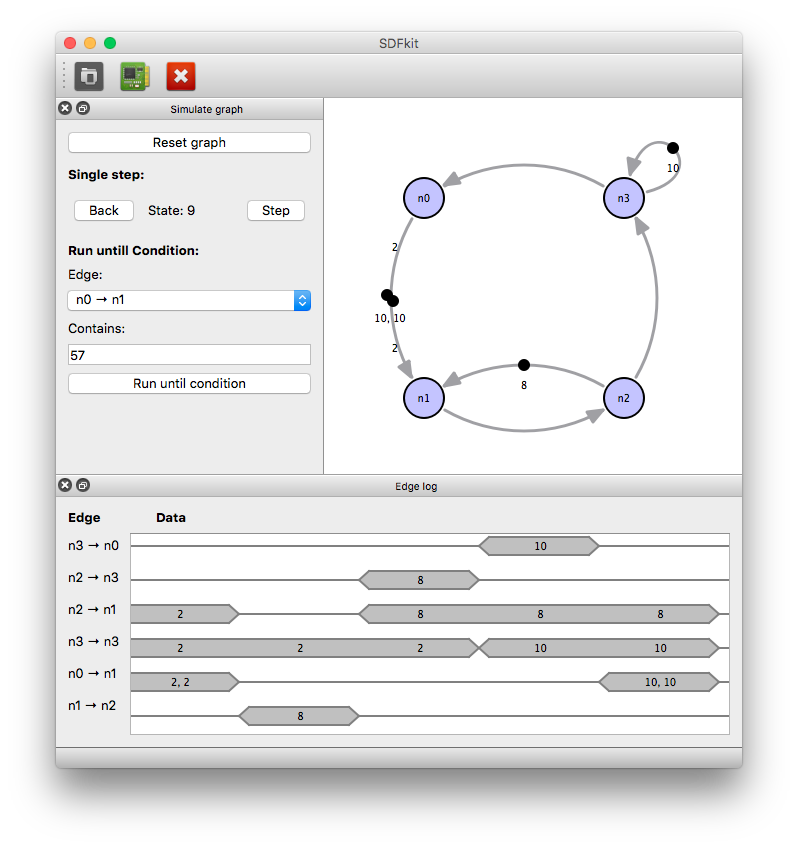
\includegraphics[width=80mm]{screenshot.png}
    \caption{Screenshot of SDFkit}
    \label{fig:screenshot}
  \end{figure}

  The central widget shows a visualization of a CSDF graph which can be simulated in a step-wise fashion using the control panel on the left.
  For debugging purposes, the data in tokens is visualized in the lower widget.

  Currently, the hardware generation backend only supports \emph{homogeneous} SDF (HSDF) graphs, which is the simplest type of SDF graph.
  The resulting generated hardware has been verified using simulation and shows the same behavior as the simulation of the HSDF graph.
  To support CSDF graphs, the edges have to support storing a variable amount of tokens each clock cycle which results in more complicated hardware.
  A stand-alone graph using a CSDF edge has been implemented and produces correct simulation results.
  Instantiation of the edges and nodes still has to be automated to complete the hardware generation for CSDF graphs.

\section{Conclusions and future work}
\label{sec:conclusions}

  In this paper we presented a methodology and an application for designing hardware using a structured approach.
  In contrast to translating imperative programming constructs like for-loops to hardware, we use constructs to express the structure in a computation.
  Using these computational structures, the generation of highly parallel hardware is tremendously simplified.
  Applications are modeled using CSDF graphs which are a cycle-accurate model for the generated hardware.
  This methodology is currently being implemented in SDFkit, an interactive simulation and hardware generation environment supporting visualization and simulation of CSDF graphs.
  Additionally, \clash\ code can be generated for HSDF graphs.

  Currently, the hardware code generation back-end is extended to support CSDF graphs.
  Additionally, the generation of a graph and transformations applied to these graph are performed in a tool outside SDFkit.
  Integration of this tool into SDFkit is therefore an other important step forward.
  Finally, interesting opportunities lie in extending the code generation with a wider range of supported platforms like C code and OpenCL.











%%% Please leave the following line as is and insert your bibliography items below.
% \begin{thebibliography}{9}\leftskip1mm\advance\labelsep\leftskip
% \bibitem{citation:1} Analog Devices: Analog Design Seminar, Munich: Analog Devices GmbH, 1989
% \bibitem{citation:2} Lancaster, Don: Das Aktiv-Filter-Kochbuch, Va- terstetten: IWT, 1986
% \bibitem{citation:3} Grütz, A.: Jahrbuch Elektrotechnik ’98,: VDE-VER- LAG, Berlin, Offenbach 1997
% \bibitem{citation:4} Huneus, H.: Lex, A.: Magnetische Eigenschaft von nichtkornorientiertem Elektroblech. etz Elektrotech.  Z. 112 (1991) H. 22, S. 1204-1208
% \bibitem{citation:5} Abramowitz, M.: Handbook of mathematical func- tions, 3rd ed., New York: Dover, 1980
% \bibitem{citation:6} Guidelines for ETEP Authors, ETEP European Transactions on Electrical Power. Vol. 7, No. 5, Sept./Oct. 1997, pp. 363-364
% \end{thebibliography}


\bibliographystyle{unsrt}
\bibliography{biblio}


\end{document}
